\documentclass[12pt]{article}\usepackage[]{graphicx}\usepackage[]{color}
% maxwidth is the original width if it is less than linewidth
% otherwise use linewidth (to make sure the graphics do not exceed the margin)

\usepackage{scrtime} % for \thistime (this package MUST be listed first!)
\usepackage[margin=1in]{geometry}
\usepackage[usenames,dvipsnames]{xcolor}
\definecolor{aqua}{RGB}{0, 128, 225}
\usepackage[colorlinks=true,citecolor=aqua,linkcolor=aqua,urlcolor=aqua,hypertexnames=false]{hyperref}
\usepackage{xspace}
\usepackage{tikz}
\usepackage{placeins} % \FloatBarrier
\usepackage{amsmath} % \text, \cases
\usepackage{enumerate} % fancier enumeration (e.g., a,b,c, ...)
\usepackage{ragged2e} % \RaggedRight
\usepackage{grffile} % \RaggedRight

%% cleveref package for convenient hyperrefercing/citing:
\usepackage[nameinlink,capitalize]{cleveref}
\crefname{equation}{Equation}{Equations}
\Crefname{equation}{Equation}{Equations}
\crefname{figure}{Figure}{Figures}
\Crefname{figure}{Figure}{Figures}
\crefname{section}{\S}{\SS}
\Crefname{section}{\S}{\SS}

%% line numbers
\usepackage{lineno}\renewcommand\thelinenumber{\color{gray}\arabic{linenumber}}

%% comments
\newcommand{\hidecomments}{\renewcommand{\comment}[3]{}}
\newcommand{\comment}[3]{\textcolor{#1}{\textbf{[#2: }\textit{#3}\textbf{]}}}
\newcommand{\david}[1]{\comment{magenta}{DE}{#1}}
\newcommand{\jd}[1]{\comment{blue}{JD}{#1}}
\newcommand{\ben}[1]{\comment{purple}{BB}{#1}}
\newcommand{\mike}[1]{\comment{orange}{ML}{#1}}

%% code
\newcommand{\code}[1]{{\tt #1}}

%% misc macros
\newcommand{\etal}{\textit{et al}.\xspace}
%% for referencing TeX macros:
\newcommand\ttbackslash{{\tt\char`\\}}
\newcommand{\macro}[1]{{\tt\ttbackslash#1}}
\newcommand{\term}[1]{{\bfseries\slshape#1}}
\newcommand{\thickredline}{{\color{red}\bigskip\begin{center}\linethickness{2mm}\line(1,0){250}\end{center}\bigskip}}

%% abbreviations
\newcommand{\ie}{\emph{i.e., }}
\newcommand{\eg}{\emph{e.g., }}
\newcommand{\etc}{\emph{etc.}\xspace}

%% notation
\newcommand{\emx}[1]{\ensuremath{#1}\xspace}
\newcommand{\R}{\emx{{\mathcal R}}}
\newcommand{\Rzero}{{\mathcal R}_0}
\newcommand{\Rt}{\emx{{\mathcal R}_t}}
\newcommand{\littler}{\emx{r}}
\newcommand{\littlerwt}{\emx{r_{WT}}}
\newcommand{\littlervoc}{\emx{r_{VOC}}}
\newcommand{\B}{\emx{\beta}}
\newcommand{\Bwt}{\emx{\beta_{WT}}}
\newcommand{\Bvoc}{\emx{\beta_{VOC}}}
\newcommand{\textsub}[2]{\emx{{#1}_{\textrm{\small #2}}}}
\newcommand{\pmob}{\textsub{p}{mob}}


%% settings
\date{\today\ @ \thistime}

\definecolor{fgcolor}{rgb}{0.345, 0.345, 0.345}
\newcommand{\hlnum}[1]{\textcolor[rgb]{0.686,0.059,0.569}{#1}}%
\newcommand{\hlstr}[1]{\textcolor[rgb]{0.192,0.494,0.8}{#1}}%
\newcommand{\hlcom}[1]{\textcolor[rgb]{0.678,0.584,0.686}{\textit{#1}}}%
\newcommand{\hlopt}[1]{\textcolor[rgb]{0,0,0}{#1}}%
\newcommand{\hlstd}[1]{\textcolor[rgb]{0.345,0.345,0.345}{#1}}%
\newcommand{\hlkwa}[1]{\textcolor[rgb]{0.161,0.373,0.58}{\textbf{#1}}}%
\newcommand{\hlkwb}[1]{\textcolor[rgb]{0.69,0.353,0.396}{#1}}%
\newcommand{\hlkwc}[1]{\textcolor[rgb]{0.333,0.667,0.333}{#1}}%
\newcommand{\hlkwd}[1]{\textcolor[rgb]{0.737,0.353,0.396}{\textbf{#1}}}%
\let\hlipl\hlkwb

\usepackage{framed}
\makeatletter
\newenvironment{kframe}{%
 \def\at@end@of@kframe{}%
 \ifinner\ifhmode%
  \def\at@end@of@kframe{\end{minipage}}%
  \begin{minipage}{\columnwidth}%
 \fi\fi%
 \def\FrameCommand##1{\hskip\@totalleftmargin \hskip-\fboxsep
 \colorbox{shadecolor}{##1}\hskip-\fboxsep
     % There is no \\@totalrightmargin, so:
     \hskip-\linewidth \hskip-\@totalleftmargin \hskip\columnwidth}%
 \MakeFramed {\advance\hsize-\width
   \@totalleftmargin\z@ \linewidth\hsize
   \@setminipage}}%
 {\par\unskip\endMakeFramed%
 \at@end@of@kframe}
\makeatother

\makeatletter
\def\maxwidth{ %
  \ifdim\Gin@nat@width>\linewidth
    \linewidth
  \else
    \Gin@nat@width
  \fi
}
\makeatother



\title{A compartmental model for epidemic parameter estimation and forecasting, with applications to SARS-CoV-2}

\author{Michael Li \and Jonathan Dushoff \and David Earn \and Irena Papst \and Benjamin M. Bolker \\
  McMaster University\\
}

\begin{document}

\linenumbers
\maketitle

\begin{abstract}
Compartmental epidemiological models are widely used to understand, manage, and forecast the SARS-CoV-2 (COVID-19) pandemic. 
We introduce a new compartmental modeling framework that shares many characteristics with existing models, but includes a number of new and noteworthy features.
In particular, it includes a flexible structure based on the \emph{flow matrix} (the \emph{per capita} rates of transitions between compartments) that allows it to be used interchangeably for discrete or continuous time and for deterministic or discrete-state stochastic models; the capacity to set starting conditions based on the expected distribution of states during an exponential phase of the epidemic; automatic computation of $R_0$ and the mean and dispersion of the generation interval for specified parameters; explicit structures incorporating the intensity of testing and delays between test administration and reporting; time-varying parameters based on breakpoints, spline bases, or external covariates such as cellphone-based mobility indices; and the ability to calibrate model parameters to multiple data streams such as case reports, hospitalization and ICU admission rates.
We demonstrate the model by calibrating it to multiple COVID-19 time series (positive tests, negative tests, hospitalizations, and deaths) for each of the Canadian provinces from 2020-02-27 to 2020-08-30.  
We estimate epidemiological parameters, including the effective reproduction number $\R_t$ over the course of the epidemic.
\end{abstract}

%%\vfill
%%\subsubsection*{Our group's COVID-19 research}
%% A brief summary, including publications by our group to date, is available at\\
%%\url{https://mac-theobio.github.io/covid-19/}.
%%\david{I updated Park et al 2020, which is now published in JRSI.  JD,
%%  please update that page with anything else you've published.}

%%\vfill

\tableofcontents

%%\vfill

%%\subsubsection*{\underline{Current date range for analysis}: \ \ date_range[1] -- date_range[2]}

%%\newpage

\section{Introduction}

SARS-CoV-2, the etiological agent of coronavirus disease 2019 (COVID-19), has been circulating in Canada since at least January 2020 \cite{onpr_200125}.
Response to the worldwide pandemic \cite{Li+20,Fauc+20} has been guided to a substantial extent by mathematical modelling \cite{Flax+20}.

%% Virological testing and contact tracing have been conducted to varying
%% degrees in different jurisdictions\david{REFS}.  While testing is
%% imperative for surveillance, its value for control is less clear.
%% Agent-based simulations indicate that the combination of testing and
%% contact tracing can be very effective in mitigating spread of
%% SARS-CoV-2 \cite{Ng+20}.  Emerging research is demonstrating that
%% saliva-based tests, as opposed to naso-pharyngeal swabs for RT-qPCR,
%% may be more effective, cheaper, and viable for the public to
%% self-administer \cite{Will+20,Wyll+20}, potentially making very
%% large-scale, frequent testing possible.

Here, we present a compartmental framework that has been developed over the course of the pandemic. 
It incorporates the standard epidemiological compartments required to model COVID-19 as well as compartments that track health-care utilization and COVID-induced
mortality. 
Case reporting can be modeled either as a time-delayed convolution of incidence or by enabling a factorial expansion of the model that accounts for the testing status of individuals \cite{Fris+20}. 
The model also allows for time-dependent variation in any rate parameter --- particularly the transmission rate --- and allows this variation to be indexed by external covariates such as cellphone-based mobility metrics, or to follow smooth (spline) curves over time. 
The same model structure can be run as an ordinary differential equation, a discrete-time-step deterministic model, or a discrete-time-step stochastic model with dynamical noise.
Finally, the model can be used to
(1) simulate specific scenarios for planning purposes;
(2) calibrate parameters to match multiple input time series such as hospital admissions or occupancy, cases, or deaths; or
(3) forecast future epidemic dynamics on the basis of past calibration.

\section{Methods}

\subsection*{Compartmental structure}

The epidemiological structure of the model is based on a susceptible-exposed-infectious-removed (SEIR) model with additional compartments reflecting the biology of COVID-19 and the structure of the health-care system. 
The COVID-19-specific compartmental structure of the model resembles many other COVID-19 models \cite{childs2021impact, tuite2020mathematical} \ben{find some refs/examples} in splitting infectious individuals into sub-compartments reflective of the epidemiology of COVID-19; it additionally adds compartments for hospitalized individuals in acute care or intensive care. 
All symptomatic individuals are presumed to have undergone a period of pre-symptomatic infectiousness (\code{p}). 
Infections can be asymptomatic (\code{a}), mildly or moderately symptomatic (\code{m}) or severely symptomatic (\code{s}); all individuals with severe symptoms go to the hospital (acute care or ICU), or die before reaching hospital (e.g., in long-term care facilities).
Some fraction of individuals who go to the ICU die. Recovered individuals (\code{R}) are assumed to be immune.  
The model includes additional compartments which facilitate book-keeping: cumulative hospital admissions (\code{X}), individuals in acute care after discharge from ICU (\code{H2}), and cumulative deaths (\code{D}) (\cref{fig:flowchart}).
(The version of the model discussed here was developed and used before vaccines were available; we have since expanded the model to include relevant compartments.)

This version of the model assumes homogeneous mixing --- all classes of infectives contribute additively to the force of infection (the \emph{per capita} infection rate of susceptibles).
We did add one feature to the model to account for heterogeneity in susceptibility in the population, which we typically imagine is driven by heterogeneity in exposure (e.g. front-line and essential workers will be infected earlier), but could also be influenced by genetic, immunological, or other factors.
A \emph{phenomenological heterogeneity} factor $\zeta$, modifies the force of infection by a factor of $\left(S(t)/N\right)^\zeta$. Since $0 < S/N < 1$, a positive value of $\zeta$ will make the force of infection decrease as the remaining fraction susceptible decreases, capturing the fact that as the most susceptible individuals are infected, they lower the average level of susceptibility in the remaining population.
\jd{Somebody said they would work on this and then hand it to me?} \ben{\cite{WilsWorc+45} uses $S^p$ but doesn't say
  anything about it: \cite{Will+06} (preceding \cite{Gran+09}) use an exponential decay rather than a power law.} \irena{DE suggested \cite{Liu+87} as well.}

%\begin{figure}[ht!]
\begin{figure}
\definecolor{shadecolor}{rgb}{0.969, 0.969, 0.969}\color{fgcolor}
\includegraphics[width=\maxwidth]{figure/flow.chart.crop.pdf}
\caption{Flow chart for basic compartmental mechanistic transmission model. 
Compartments: \code{S} (susceptible), \code{E} (exposed), \code{Ia} (asymptomatic infection), \code{Ip} (presymptomatic infection), \code{Im} (mild/moderately symptomatic infection), \code{Is} (severely symptomatic infection), \code{H} (hospitalized [acute care]), \code{ICUs} (ICU with prognosis of survival), \code{ICUd} (ICU with prognosis of death), \code{H2} (acute care after ICU stay). 
Compartments denoted by rectangles are accumulators, primarily used in the condensation step to compute incidences: \code{R} (recovered), \code{D} (dead), \code{X} (accumulator for cumulative hospital admissions).
\ben{prettify this further, \textbf{or} steal something better from Irena?}}
\label{fig:flowchart}
\end{figure}

%% \begin{figure}[ht!]
%% \definecolor{shadecolor}{rgb}{0.969, 0.969, 0.969}\color{fgcolor}
%% \includegraphics[width=\maxwidth]{figure/ratematrix.pdf}

%% \caption{Flow matrix for basic compartmental mechanistic transmission
%%   model.  Gray indicates non-zero flows: compartments as in
%%   \cref{fig:flowchart}.  \ben{do we want this? It's equivalent to
%%     the flowchart, could be used to show differences in magnitude (via shading)
%%   if we sorted out the details} \jd{I think we don't.}
%%   }
%% \label{fig:flowmatrix}
%% \end{figure}

Internally, the model is defined by a \emph{flow matrix} $\mathbf{M}$, whose elements specify the \emph{per capita} rates at which individuals move from one compartment to another.
For the basic model, the only element of the flow matrix that needs to be recomputed at each time step is the incidence (flow from $S$ to $E$); all other rates are constant except when the model specifies a piecewise change.

This set-up allows for considerable flexibility.
\begin{itemize}
\item For a numerical differential equation solver, we need the time derivatives of each compartment. The absolute rates are computed by columnwise multiplication by the state vector $\mathbf s$ (${\mathbf F}_{ij} = \mathbf{M}_{ij} \mathbf{s}_j$).
The gradient is the difference between the total flows into (column sums of $\mathbf F$) and out of (row sums of $\mathbf F$) each compartment.
\item For a discrete-time model, we compute the vectors of outflows and inflows as above, but simply compute the new states as (original state + (inflow - outflow)$\Delta t$).
\item We can also use a discrete-time model with a \emph{hazard correction} to the flows to address the possibility that a state will go negative due to an overly large outflow. Instead of the total \emph{per capita} outflow of a compartment being equal to the sum of \emph{per capita} flow to each other compartment ($\textsub{f}{tot} = \sum_i {\mathbf M}_{ij}$), we let the total outflow be $\textsub{f'}{tot} = 1-\exp(-\textsub{f}{tot} \Delta t)$; the individual flows are then adjusted by a factor of $\textsub{f'}{tot}/\textsub{f}{tot}$.
This adjustment accounts for the effects of depletion during the course of a time step.
\item Finally, if we choose to run a fully stochastic simulation, the flow matrix $\mathbf M$ is what we need to sample the flows between compartments as Euler-multinomial deviates \cite{breto+09}, which take the hazard correction described above and use it to compute probabilities for draws from binomial or multinomial random deviates.
\end{itemize}

While the flow matrix description is convenient for most epidemiological dynamics, there are a few epidemiological processes that are more naturally captured by absolute rather than \emph{per capita} rates, for example (1) when intensities of public health interventions such as numbers of tests or vaccines administered are reported by public health agencies; or (2) in models incorporating births or immigration.
We have typically handled the former case by taking observed vaccination or testing rates and dividing them by current compartment sizes in order to set the relevant entries in the flow matrix; we have not yet tried to build models including inflows from outside the system (the latter case).
\mike{Nothing wrong with adding vaccination here, but do we want to stick with it or remove it given we didn't do it for this paper?} \ben{think it's fine}

We typically compute the model dynamics deterministically, as a discrete-time model with a hazard correction (the third option above).  Once the trajectories are computed, we reduce the full state vector to a more convenient, collapsed state vector in a step we call \emph{condensation}, for example by summing all of the infectious compartments to a single $I$ state vector, or collapsing the different acute-care ($H$, $H2$) or ICU ($\textrm{ICU}_s$, $\textrm{ICU}_d$) compartments.
As well as allowing us to visualize model results more conveniently, condensation also allows us to compare the simulated state vector to available data streams.
In addition to summing compartments, we can also compute incidences as time-lagged differences of accumulator compartments (for example, differencing accumulated deaths $D$ to derive a mortality rate) or perform more complicated operations such as convolution. 
Our main use of convolution is to convert incidence, which we compute by multiplying the force of infection by the number of susceptibles, to a case-reporting time series: $\textrm{CR}(t) = \sum \phi(i) (\textrm{FOI}(t-i) S(t-i))$, where we typically set $\phi(i)$ to be a Gamma distribution with
moments chosen to match estimates of case-reporting delays
\ben{how did we pick these values? 
Probably don't have a formal ref but some statement of what we used to guess that this was reasonable would be good ...}.
\jd{Another option here would just be to say where $\phi$ is typically a Gamma distribution with moments chosen to match literature estimates>}
\ben{done, but still not clear that there are a lot of such estimates in the literature \ldots}
When computing case reports from incidence we also include a case-report proportion \code{c\_prop} to account for the fact that the majority of COVID infections are never reported \cite{Doug+2020}; this value is usually calibrated from data.

Once condensation is done, the model also allows us to add observation error, which we typically simulate from a negative binomial distribution with a variable-specific dispersion parameter.

\subsection*{Expansion to accomodate testing}

At the cost of additional complexity, we can add explicit testing compartments to the model.
In the simpler version of the model, we assume that a specified fraction of infections are reported as cases (or calibrating this value from joint data on cases and hospitalizations), and imposing a distributed delay between infection and reporting (i.e. via convolution).
Here we instead expand the susceptible and all infected compartments factorially to include the possibilities that individuals in those epidemiological classes are untested; tested and awaiting negative results; tested and awaiting positive results; or tested positive.
After receiving negative results (whether true negatives, from individuals in $S$, or false negatives, from individuals in one of the infectious compartments), individuals cycle back to the untested sub-compartment where they can be tested again. After receiving positive results, they remain in the positively tested sub-compartment; depending on the model parameters, their transmission may be reduced due to self-isolation (controlled by the parameter \code{iso\_t}); we assume here that people waiting for test results do not isolate.
\cite{Ghar+22} thoroughly analyze the epidemiological consequences of this structure in a simpler framework that uses a simple SIR model rather than the COVID-specific compartmental model (\cref{fig:flowchart}) as the foundational epidemiological model.
Individuals may progress between epidemiological compartments (e.g., becoming infectious or recovering) while awaiting the results of tests. In general, progressing individuals move to the same testing subcompartment (e.g., from \code{Im}, negative-waiting to \code{R}, negative-waiting).

We define a weight vector $w$ across epidemic compartments that gives weight $w_a$ to asymptomatic classes (\code{S}, \code{E}, \code{Ia}, \code{Ip}, \code{R}) and 1 to symptomatic classes (i.e., all other classes).
If $W$ is the weighted sum of compartment occupancies $X_i$ (i.e., $\sum_i w_i X_i/N$), then for a daily \emph{per capita} testing rate $\rho$ we might expect that the corresponding \emph{per capita} testing rate in compartment $i$ would be $T_i = \rho w_i/W$. 
However, under some extreme conditions (if testing is so extreme that few untested symptomatic people are left) this formulation can allow the \emph{per capita} testing rate to explode. To mitigate this problem we add a maximum daily \emph{per capita} testing rate $\tau$ to the model such that
\[T_i = \frac{\rho \tau w_i}{\tau W + \rho} .\] (see \cite{Ghar+22} appendix A.5 for more details).
The testing flows out of each untested subcompartment are divided into flows to ``positive waiting'' and ``negative waiting'' compartments according to the infection status of the relevant compartment and specificity/sensitivity parameters. If tests are assumed to be perfectly specific and sensitive, then all individuals from non-infectious compartments (\code{S}, \code{E}, \code{R}) enter the ``negative waiting'' and those from infectious compartments enter the ``positive waiting'' compartment.

We assume that all individuals admitted to the hospital for COVID-19 are immediately tested. (These tests are not included in the accounting of test distribution above, but in the COVID setting they represent a small fraction of the overall number of tests administered.)

\begin{figure}
  \includegraphics{figure/testFlow.1.Rout.pdf}
  \caption{Testing flow. Every epidemiological compartment is subdivided into the four subcompartments shown.
    Black arrows represent flows between subcompartments due to testing processes (test administration, reporting of tests); blue arrows represent progression between epidemiological compartments.
    Dashed arrows represent the accumulation of negative and positive test reports, which can be compared against data.
    \ben{is there a better version of this somewhere?}}
	 \mike{Irena}
  \label{fig:testing_flow}
\end{figure}

\subsection*{Model parameterization}

The model allows for time-varying, piecewise-constant changes in any parameter. 
Our early analyses focused on changes in time-varying effective reproductive number (\Rt) due to behaviour change and non-pharmaceutical interventions, which we model by changing the transmission rate.
The transmission rate $\beta(t)$ is taken to be a time-varying function of the form $\beta_0 \beta_1(t)$ where $\beta_0$ is the baseline value for transmission from symptomatic individuals.
Individuals in different symptomatic classes (presymptomatic, asymptomatic, mild, severe) may have their transmission modified by a specified multiplier (given as model parameters); we assume that hospital transmission is negligible.
The time-varying (relative) transmission $\beta_1$ can incorporate a variety of different effects, one at a time or in combination:
\begin{itemize}
\item abrupt (piecewise) changes on specified dates when control measures are known to have been implemented;
\item proportional to a power of observed mobility or some other exogenous proxy for contact behaviour
\[
  \beta_1(t) \propto (\textrm{relative mobility})^{\pmob}
\]
for some power $\pmob>0$;
\item according to an arbitrary spline curve, i.e. a linear combination of components of a B-spline basis.
\end{itemize}

All of the sub-models for temporal change in the transmission rate can be subsumed under a single log-linear model:
\begin{equation}\label{eq:betamodel}
\log \beta(t) = \log \beta_0 + \boldsymbol{X}\boldsymbol{c}
\,,
\end{equation}
where $\boldsymbol{X}$ is a model matrix that can contain any combination of covariates and $\boldsymbol{c}$ is a vector of covariates determining differences in the log of the relative transmission rate.
In particular, piecewise breaks correspond to indicator variables for which period an observation falls in; the mobility model corresponds to a column containing the log of relative mobility; and the spline model corresponds to a set of columns containing the basis vectors of a B-spline basis with specified knots.

In practice, when we use the model without incorporating covariates we adopt a simpler strategy of providing a list of the breakpoints and the parameters that change at those breakpoints --- a special case of the more general log-linear model. When we fit the model with 

\mike{Add something here about the mobility set up? Different intercepts and slopes + a smoother}

\subsection*{Derived parameters and parameter setting}

It is useful to be able to compute several quantities derived from the parameters of a model, in particular (1) the dominant eigenvector of the system in the exponential growth phase; (2) the value of \Rzero and the intrinsic growth rate $r$; (3) the mean and coefficient of variation of the generation interval. 
In principle we could compute these values directly from the flow matrix, by constructing the Jacobian matrix and the next-generation matrix and performing the appropriate eigenvector/eigenvalue calculations (as discussed by \cite{VandWatm02} for differential equations and \cite{Casw00} for discrete-time systems). However, we found it simpler to derive these values by simulation.

To compute the eigenvector, we run a simulation where we set the outflow from the susceptible compartment to zero (while maintaining the \emph{inflow} from $S$ to $E$), which mimics the dynamics near the disease-free equilibrium where susceptible depletion is negligible. After running the simulation for a long time (100 steps by default), the state vector is close to the eigenvector.  
We use this value to set starting conditions when starting near the beginning of the epidemic. 
It is easy to specify a scalar value (say, 1\% of the population) to indicate the initial size of the epidemic; by distributing these individuals according to the calculated eigenvector, we reduce numerical instability at the beginning of our simulations. 

To compute the other summaries (\Rzero, $r$, and moments of the generation interval) we rely on the fact that the software saves the force of infection at each time step. 
We simulate the progression of a \emph{single} individual through the infection process, i.e. setting the population size to 1 and setting the initial state to $E=1$ with all other compartments empty. 
Simulating deterministically then generates a time course of the probability that an individual is in any given box at a particular age of infetion, and thus also the expected force of infection generated by a single infectious individual, as a function of time since infection. 
This vector $K(t)$ is the same as the transmission kernel in a renewal equation \cite{Cham+18}. 
We can easily compute $\Rzero = \sum_t K$, mean generation interval  $\bar G = \sum_t K(t)/\Rzero \cdot t$, and generation interval coefficient
\[
\textrm{CV}(G) = \frac{\sqrt{\sum_t K(t)/\Rzero (t- \bar G)^2}}{\bar G} .
\]
The growth rate $r$ can be computed by numerically solving the Euler-Lotka equation
\[
\sum_t  K(t) e^{-r t} = 1
\]
for $r$.

\jd{Suggest dropping the detailed equations for Gbar and CV, but instead adding $g(t)$ and saying that we also calculate its mean and CV.}

\jd{Suggested easy ref is ChamDush15: http://dx.doi.org/10.1098/rspb.2015.2026 (instead of current Cham18)}

\ben{check: what do we do about phenom het/$\zeta$ in these procedures, esp about incorporating it in any computation of \Rt?}

\jd{$\zeta$ should not pose any special problems here; when $S\approx N$ its effect is negligible. At other times (if any), it should be handled correctly by setting $S$ and $N$ correctly and suppressing outflow from $S$ as described.}

In addition to its use in summarizing a given set of parameters, the computation of $\Rzero$, $r$, and the generation interval is useful as an initial step in calibrating the model. 
Estimates of these summary statistics are more broadly available \cite{park2020reconciling}, and more epidemiologically relevant, than the more specific mechanistic parameters describing the relative infectiousness and duration of each of the different infectious compartments (although this detailed information is still important for determining the effectiveness of interventions like contact tracing). 
We typically start with mechanistic parameters gathered from the literature and pre-calibrate them to specified target values of $r$ (which is easy to estimate from the observed initial growth rate of the epidemic in a region) and the mean generation interval by adjusting $\beta_0$ (baseline transmission) and simultaneously scaling the values of all of the epidemiological transition rates ($\sigma$, \textsub{\gamma}{s}, \textsub{\gamma}{m}, \textsub{gamma}{a}) by a single factor until the target values are achieved.

\subsubsection*{Calibration}

Once we have run a deterministic model simulation for a particular set of parameters (including a starting number infected, distributed across non-susceptible classes according to the exponential-phase eigenvector computed as described above) and we have some set of time series data to calibrate against (for example, case reports and hospital admissions), we can calculate a log-likelihood. 
We assume that every observation is independently negative binomially distributed, with a series-specific estimated dispersion parameter (i.e. the variability in cases, hospital admissions, etc. will differ). 
We use standard nonlinear optimization algorithms built into R, such as Nelder-Mead, to find the maximum likelihood estimates; when we have had difficulty with numerical instability, we have performed an initial fit with differential evolution \cite{Mull+11} followed by a final fit with Nelder-Mead.

A link function can be added for any parameter in the model to constrain it to a sensible domain; the user specifies this by adding an appropriate prefix to the name of the parameter in the list of starting values for parameters to be calibrated. 
For example, specifying \code{log\_beta0 = -1} would specify that the baseline transmission parameter $\beta_0$ should be calibrated on the log scale, ensuring that the value of $\beta_0$ is always positive, and using a starting value of -1 on the log scale (i.e. initial $\beta_0 = \exp(-1)$). 
Specifying \code{logit\_nonhosp\_mort = -0.2} would specify that the value of \code{nonhosp\_mort} (the fraction of non hospitalized mortality) should be fitted on a logit, or log-odds, scale, ensuring that it is bounded between 0 and 1, and using a starting value of $\beta_0 = \textrm{logit}^{-1}(-0.2) = 0.45$.

The model includes a general framework for adding a prior probability distribution for any parameter, using any distribution available in R. 
For example, \code{dbeta(nonhosp\_mort, 2, 2)} would specify a $\textrm{Beta}(2,2)$ prior for \code{nonhosp\_mort}.
We do not need to adopt a fully Bayesian framework to make use of priors; instead, we can think of them as convenient regularizing factors to keep the model-fitting process numerically stable. If we do want to be Bayesian, then the fitting procedure described above will return maximum \emph{a posteriori} (MAP) parameter values, not a sample from the full posterior distribution as is standard with frameworks that use Markov chain Monte Carlo.


In Ontario, we calibrate to deaths, and new confirmations, all of which are available publicly. 
In the expanded model, we can include time series of both positive and negative tests in our calibration. 
Reported new confirmations are the most reliable and voluminous source of epidemic information.
Unfortunately, they are also subject to many inherent biases, including substantial variation over time in \term{testing intensity} (\ie tests \emph{per capita} per day).

We simultaneously estimate the temporal pattern of the transmission rate [Equation~\eqref{eq:betamodel}] \mike{two mobility intercept and three slopes}, and several basic model parameters (\cref{estparmtab}) \mike{E0(initial number of exposed), beta0, nonhosp\_mort, zeta(pheomhet), dispersion parameters (report and death)}.
\mike{how does cref work?}
Other model parameters are taken from the literature (\cref{litparmtab}).
\ben{need more details: which parameters are estimated? what are the
  rules about breakpoints? Are we using mobility, phenom het, etc., or not?}
\mike{everything else from ON.csv, the main ones are hospital parameters given we are not calibrating to them, and the time spent in each box.}

We do not include hospitalization and ICU occupancy in our calibration because our model assumes all severe cases go through ICU, whereas many severe cases actually occur entirely in Long Term Care Facilities (LTCFs) and capacities limitations. 
\ben{not sure what this means; is this really the reason that we exclude ICU, or do we exclude it because the data are wonky? Before we added the non-hospital mortality flow, this would have been a reason not to calibrate to \emph{deaths}, but otherwise I don't understand this \ldots}
\mike{this is weird now. If we don't calibrate to hospitalization at all, calibrating to death will not make sense. Drop it and calibrate to reports only?}

\ben{commented out section on estimation of $R_t$, covered above --- and
  analytic expressions are less general than the kernel machinery}
%% \hypertarget{Rt}{}
%% \subsubsection*{Estimation of effective reproduction number $\R_t$}

%% The basic reproduction number for the basic model is (\emph{cf.}\/
%% \cref{litparmtab,estparmtab}) \david{I took this from the vignette,
%%   where I wrote it months ago.  Are we just setting
%%   $\texttt{iso}_{\rm m,s}=0$?} \ben{(1) Yes; we could include the isolation
%%   parameters if we wanted, but we have yet to set them to anything
%%   other than zero. (2) Why are the subscripts for infection
%%   category (a,m,p) Roman rather than math italic?}
%% %%
%% %% \begin{equation}\label{eq:R0}
%% %% \R_0 = \beta_0 \left\{
%% %% \alpha \frac{C_{\rm a}}{\gamma_{\rm a}}
%% %% +
%% %%  (1-\alpha)\left[ \frac{C_{\rm p}}{\gamma_{\rm p}}
%% %%   + \mu(1-\texttt{iso}_{\rm m})\frac{C_{\rm m}}{\gamma_{\rm m}}
%% %%   + (1-\mu)(1-\texttt{iso}_{\rm s})\frac{C_{\rm s}}{\gamma_{\rm s}} \right]
%% %%   \right\} \,.
%% %% \end{equation}
%% \begin{equation}\label{eq:R0}
%% \R_0 = \beta_0 \left\{
%% \alpha \frac{C_{\rm a}}{\gamma_{\rm a}}
%% +
%% (1-\alpha)\left[ \frac{C_{\rm p}}{\gamma_{\rm p}}
%%   + \mu\frac{C_{\rm m}}{\gamma_{\rm m}}
%%   + (1-\mu)\frac{C_{\rm s}}{\gamma_{\rm s}} \right]
%%   \right\} \,.
%% \end{equation}
%% For the full model (including testing flows), we compute $\R_0$
%% numerically via \cite{WallLips07}
%% \begin{equation}
%% \frac{1}{\R_0} = \int_0^\infty e^{rt} g(t)\,{\rm d}t \,,
%% \end{equation}
%% where the exponential growth rate is obtained by solving the model
%% linearized about the disease-free equilibrium \cite{Ma+14}, and the
%% generation interval distribution is obtained by solving the cohort
%% equations associated with the model (\emph{cf.}\/
%% \cite{Cham+18}).\david{Did I correctly describe what we are actually
%%   doing?}\david{We should state the numerical value of $\R_0$, with
%%   and without testing flows.  Or are we adjusting it with
%%   \code{\detokenize{fix_pars}} anyway?  If the latter, we need to
%%   explain that.}
%% %%
%% The effective reproduction number at time $t$ is
%% \begin{equation}\label{eq:Rt}
%% \R_t = \R_0\, \beta_1(t) \Big(\frac{S(t)}{N}\Big)^{1+\zeta}\,.
%% \end{equation}

\subsubsection*{Forecasting}

Our calibrations yield values for the parameters of our deterministic model. 
Using the calibrated parameters, we generate 1000 multivariate normal sets of parameters and feed it into the deterministic model to generate an ensemble of forecast. We extend the end date of the calibration window (i.e. the last observed data point for calibration) to create a forecast window. Inside the forecast window, the user either input non-calibrated data (i.e. mobility, testing and etc) or assumed the last set of inputs and calibrated parameters be constant throughout the forecasting window. 
\mike{Please check guts and see if it is doing this.}

\subsection{Data sources}

\david{This section describes all the data available to us, whether we
  use it or not.  This is harmless for the PHAC report, but we'll need
  to describe only data we when we submit for publication.}
\mike{I am commenting out all the parts we are not using}
% 
% One of us (ML) maintains a public web site containing Canadian
% COVID-19 data at the provincial level.  Data are frequently downloaded
% from a variety of sources and cleaned.  See
% \url{https://wzmli.github.io/COVID19-Canada/}.
% 
% While the public data do include line lists of records for individual
% patients, there are several important limitations:
% \begin{itemize}
% \item A single \term{episode date} is given, with no indication of
%   whether this refers to the date of onset of symptoms, date of
%   testing, date of report, \emph{etc.}
% \item Only a broad age class is given (\eg 50--59), rather than the
%   exact age of each patient.
% \end{itemize}

\mike{let's stick with public Ontario for now?}
\subsubsection*{Public COVID-19 data for Ontario, Canada}


Daily reported data on COVID-19 testing and outcomes (confirmed cases, death, hospital and ICU occupancy) in Ontario are publicly available from the official provincal website. See
\url{https://data.ontario.ca/dataset/f4f86e54-872d-43f8-8a86-3892fd3cb5e6/resource/ed270bb8-340b-41f9-a7c6-e8ef587e6d11/download/covidtesting.csv}.

However, this dataset does not have testing counts before April 15th. 
One of us (ML) maintains a public web site containing Canadian COVID-19 data at the provincial level since the beginning of the COVID-19 pandemic.   
Data are frequently downloaded from a variety of sources and cleaned.  See
\url{https://wzmli.github.io/COVID19-Canada/}.

% \subsubsection*{Detailed COVID-19 data for Ontario}

% Through Public Health Ontario
% (\href{https://www.publichealthontario.ca/}{PHO}), we have obtained access to
% data from a number of health databases.
% \begin{description}
% \item[iPHIS]A line list extracted from the integrated Public Health
%   Information System
%   (\href{https://www.publichealthontario.ca/en/diseases-and-conditions/infectious-diseases/ccm/iphis}{iPHIS})
%   includes, for most patients:
%   \begin{itemize}
%   \item dates of symptom onset, specimen collection, case report, ER
%     visit, hospital admission and discharge, ICU admission and
%     discharge, death;
%   \item gender;
%   \item either age (in two-year age groups) OR location (FSA: first
%     three characters of postal code).
% 
%   \end{itemize}
% \item[OLIS]A line list extracted from the Ontario Laboratories
%   Information System
%   (\href{https://www.ehealthontario.on.ca/en/for-healthcare-professionals/ontario-laboratories-information-system-olis}{OLIS})
%   provides information on every COVID-19 test performed in Ontario.
%   (The records are unfortunately not linked to the iPHIS database.)
%   Age is given only in 10-year age classes.
% \item[ICES]Through a secure data portal at
%   \href{https://www.ices.on.ca/}{ICES}, we can access more complete
%   data from
%   \href{https://www.ehealthontario.on.ca/en/for-healthcare-professionals/ontario-laboratories-information-system-olis}{OLIS}
%   (including age rather than age group of each tested individual), the
%   Discharge Abstract Database
%   (\href{https://www.cihi.ca/en/discharge-abstract-database-metadata}{DAD}),
%   the National Ambulatory Care Reporting System
%   (\href{https://www.cihi.ca/en/national-ambulatory-care-reporting-system-metadata}{NACRS})
%   and claims made to the Ontario Health Insurance Plan
%   (\href{https://www.ontario.ca/page/what-ohip-covers}{OHIP}).  These
%   databases are linkable through encrypted individual identifiers.
%   \david{Is iPHIS definitely not available within ICES?}
% 
%   Using the ICES secure data portal is awkward and time-consuming;
%   other than conducting some exploratory analysis, we have so far used
%   it only to obtain the detailed age structure of the OLIS testing
%   data (which is not available to us via iPHIS).
% \end{description}



\hypertarget{Mobility data}{}
\subsubsection*{Mobility data}

We use mobility data from
Apple\footnote{\url{https://raw.githubusercontent.com/ActiveConclusion/COVID19_mobility/master/apple_reports/applemobilitytrends.csv}}
and
Google\footnote{\url{https://www.gstatic.com/covid19/mobility/Global_Mobility_Report.csv}}
for each province as a whole. From these data we derive a
\term{relative mobility index} using the ``driving'' index from Apple
and the ``retail and recreation'' and ``workplaces'' indices from
Google; we compute a 7-day moving average of these indices, rescale
all of them to have a baseline (pre-pandemic) value of 1.0, and
average the three indices (equally weighted), to obtain an overall
index for each day.

% \subsubsection*{Important dates}
% 
% Our code allows us to model abrupt effects on the effective
% reproduction number ($\R_t$) on a given set of dates, and to find the
% relative transmission changes that best fit the data.
% 
% Key dates in Ontario are listed in \cref{tab:dates}.  We ignore the
% initial declaration of emergency on 17 March 2020 because this
% occurred during the March Break for schools and therefore had a small
% effect until 23 March when schools would have re-opened and workplaces
% were ordered to close.  Many other measures, announcements and
% developments are listed (for each province and territory) in the
% document \texttt{Timeline of FPT PH Measures on COVID-19
%   2020-05-04.docx} provided by the Chief Science Advisor on 8 May
% 2020. \david{That statement is fine for the report, but not for a
%   publication.} However, for Ontario, there are no other obvious dates
% that seem to be likely to be associated with a major change in social
% distancing.
% 
% \david{Ontario covid timeline from Wikipedia: \url{https://en.wikipedia.org/wiki/COVID-19_pandemic_in_Ontario}.}
% 
% We have chosen not to fit abrupt changes in $\R_t$ because we have
% found that \hypertarget{Mobility data}{relative mobility indices}
% yield more plausible fits.  Mobility indices seem to better reflect
% (1) gradual uptake/compliance with discrete changes in government
% policies, and (2) behavioural changes that are not directly related to
% official policies.
% 
% \begin{table}[ht]
% \begin{center}
%   \RaggedRight
%   \renewcommand{\arraystretch}{1.5}
%   \small
% \begin{tabular}{ c | p{7cm} | p{6cm} }
% {\bfseries Date} & {\bfseries Event} & {\bfseries Comment} \\ \hline
% 
% 11 March 2020 &
%                 \href{https://www.who.int/dg/speeches/detail/who-director-general-s-opening-remarks-at-the-media-briefing-on-covid-19---11-march-2020}{W.H.O.~declares COVID-19 pandemic} \\
% 17 March 2020 &
%                 \href{https://news.ontario.ca/opo/en/2020/03/ontario-enacts-declaration-of-emergency-to-protect-the-public.html}{Ontario
%                 declares emergency} & Schools ordered to stay
%                                             closed after March Break. \\
% 23 March 2020 & Ontario orders workplaces to close & Initially
%                                                     \href{https://news.ontario.ca/opo/en/2020/03/ontario-closing-at-risk-workplaces-to-protect-health-and-safety.html}{At-Risk
%                                                     Workplaces} and
%                                                     then
% \href{https://news.ontario.ca/opo/en/2020/03/ontario-orders-the-mandatory-closure-of-all-non-essential-workplaces-to-fight-spread-of-covid-19.html}{All
%                                                     Non-Essential
%                                                     Workplaces}. \\
% 
% 28 March 2020 &
%                 \href{https://news.ontario.ca/opo/en/2020/03/ontario-prohibits-gatherings-of-five-people-or-more-with-strict-exceptions.html}{Ontario
%                 restricts gatherings} & Gatherings of more than five
%                                         people prohibited, with strict exceptions.\\
% 19 May 2020 &
%               \href{https://www.ontario.ca/page/reopening-ontario-whats-each-stage#section-1}{Ontario
%               entered Stage 1 of reopening} & \\
% 12 June 2020 &
%                \href{https://www.ontario.ca/page/reopening-ontario-whats-each-stage#section-2}{Most
%                public health unit regions allowed to move into Stage
%                2 (not Peel and Toronto)} & Restaurants and bars can open for dining in outdoor areas only.\\
% 24 June 2020 &  Peel and Toronto entered Stage 2& \\
% 17 July 2020 &  Some regions entered Stage 3& \\
% 31 July 2020 &  Peel and Toronto entered Stage 3& \\
% 12 August 2020 & Windsor-Essex entered Stage 3& \\
% \end{tabular}
% \end{center}
% \caption{Key dates in Ontario.}
% \label{tab:dates}
% \end{table}
% 
% \bigbreak \bigbreak \bigbreak
% % The data we use to calibrate our dynamical models are shown in \cref{fig:data}.
% % \begin{figure}
% 
% %% \caption{The daily Ontario COVID-19 data that we use to calibrate our
% %%   models: number of COVID-19 deaths (death), number of COVID-19
% %%   patients currently in acute care in hospital (H), number of COVID-19
% %%   cases reported (report).  Reporting began on date_range[1].
% %%   The most recent counts are for date_range[2].  The bottom
% %%   panel shows an index of mobility derived from cell phone data
% %%   collected by Google and Apple.  The thick grey line shows the date
% %%   the COVID-19 data begin, the red solid line shows the date that the
% %%   WHO declared a COVID-19 pandemic (11 March 2020), the red dotted
% %%   line shows the date of the Declaration of Emergency in Ontario (17
% %%   March 2020), and the grey dotted line shows the date on which
% %%   workplaces were ordered closed in Ontario (23 March 2020).}
% %%   \label{fig:data}
% %% \end{figure}
% \david{Caption to old figure is commented out.  Possibly useful at some
% point.}

\FloatBarrier

\hypertarget{sec:Results}{}
\section{Results}

\mike{Do we want to include some simulation to show the model works and can do the calibration?}
\mike{figure captions and make better plots}

\subsection{Base model}

Figure \ref{fig:Ont_calibration} shows the fit to data of a basic model that calibrates to COVID new cases and death for Ontario from February 24, 2020 (the first covid case reported in Ontario) to August 30, 2020. 
\mike{do we need a justification of the end date?}
The basic model was chosen to be the base model because reported cases and death time series are most commonly applicable to public data for many juristrictions.
This time frame captures the first wave of the COVID outbreak in Ontario. 
We did not explicitly include break dates (i.e. time-varying transmission rates) to match different public health measures and restrictions in place within the fitting window, the transmission rate is a function of time-varying intercepts and slopes on mobility index which is a sensible proxy for changes in behaviour responding to public health restrictions.
Hospital occupancy and death on the other hand does not fit to the data well after the initial wave. This suggest the proportion hospitalized and death are lower and should be time varying as well. 


\begin{figure}[ht!]
\definecolor{shadecolor}{rgb}{0.969, 0.969, 0.969}\color{fgcolor}
\includegraphics[width=\maxwidth]{figure/ontario_mobility.png}

\caption{Ontario mobility}
\label{fig:Ont_mobility}
\end{figure}

\mike{keep only forecast plot?}


\begin{figure}[ht!]
\definecolor{shadecolor}{rgb}{0.969, 0.969, 0.969}\color{fgcolor}
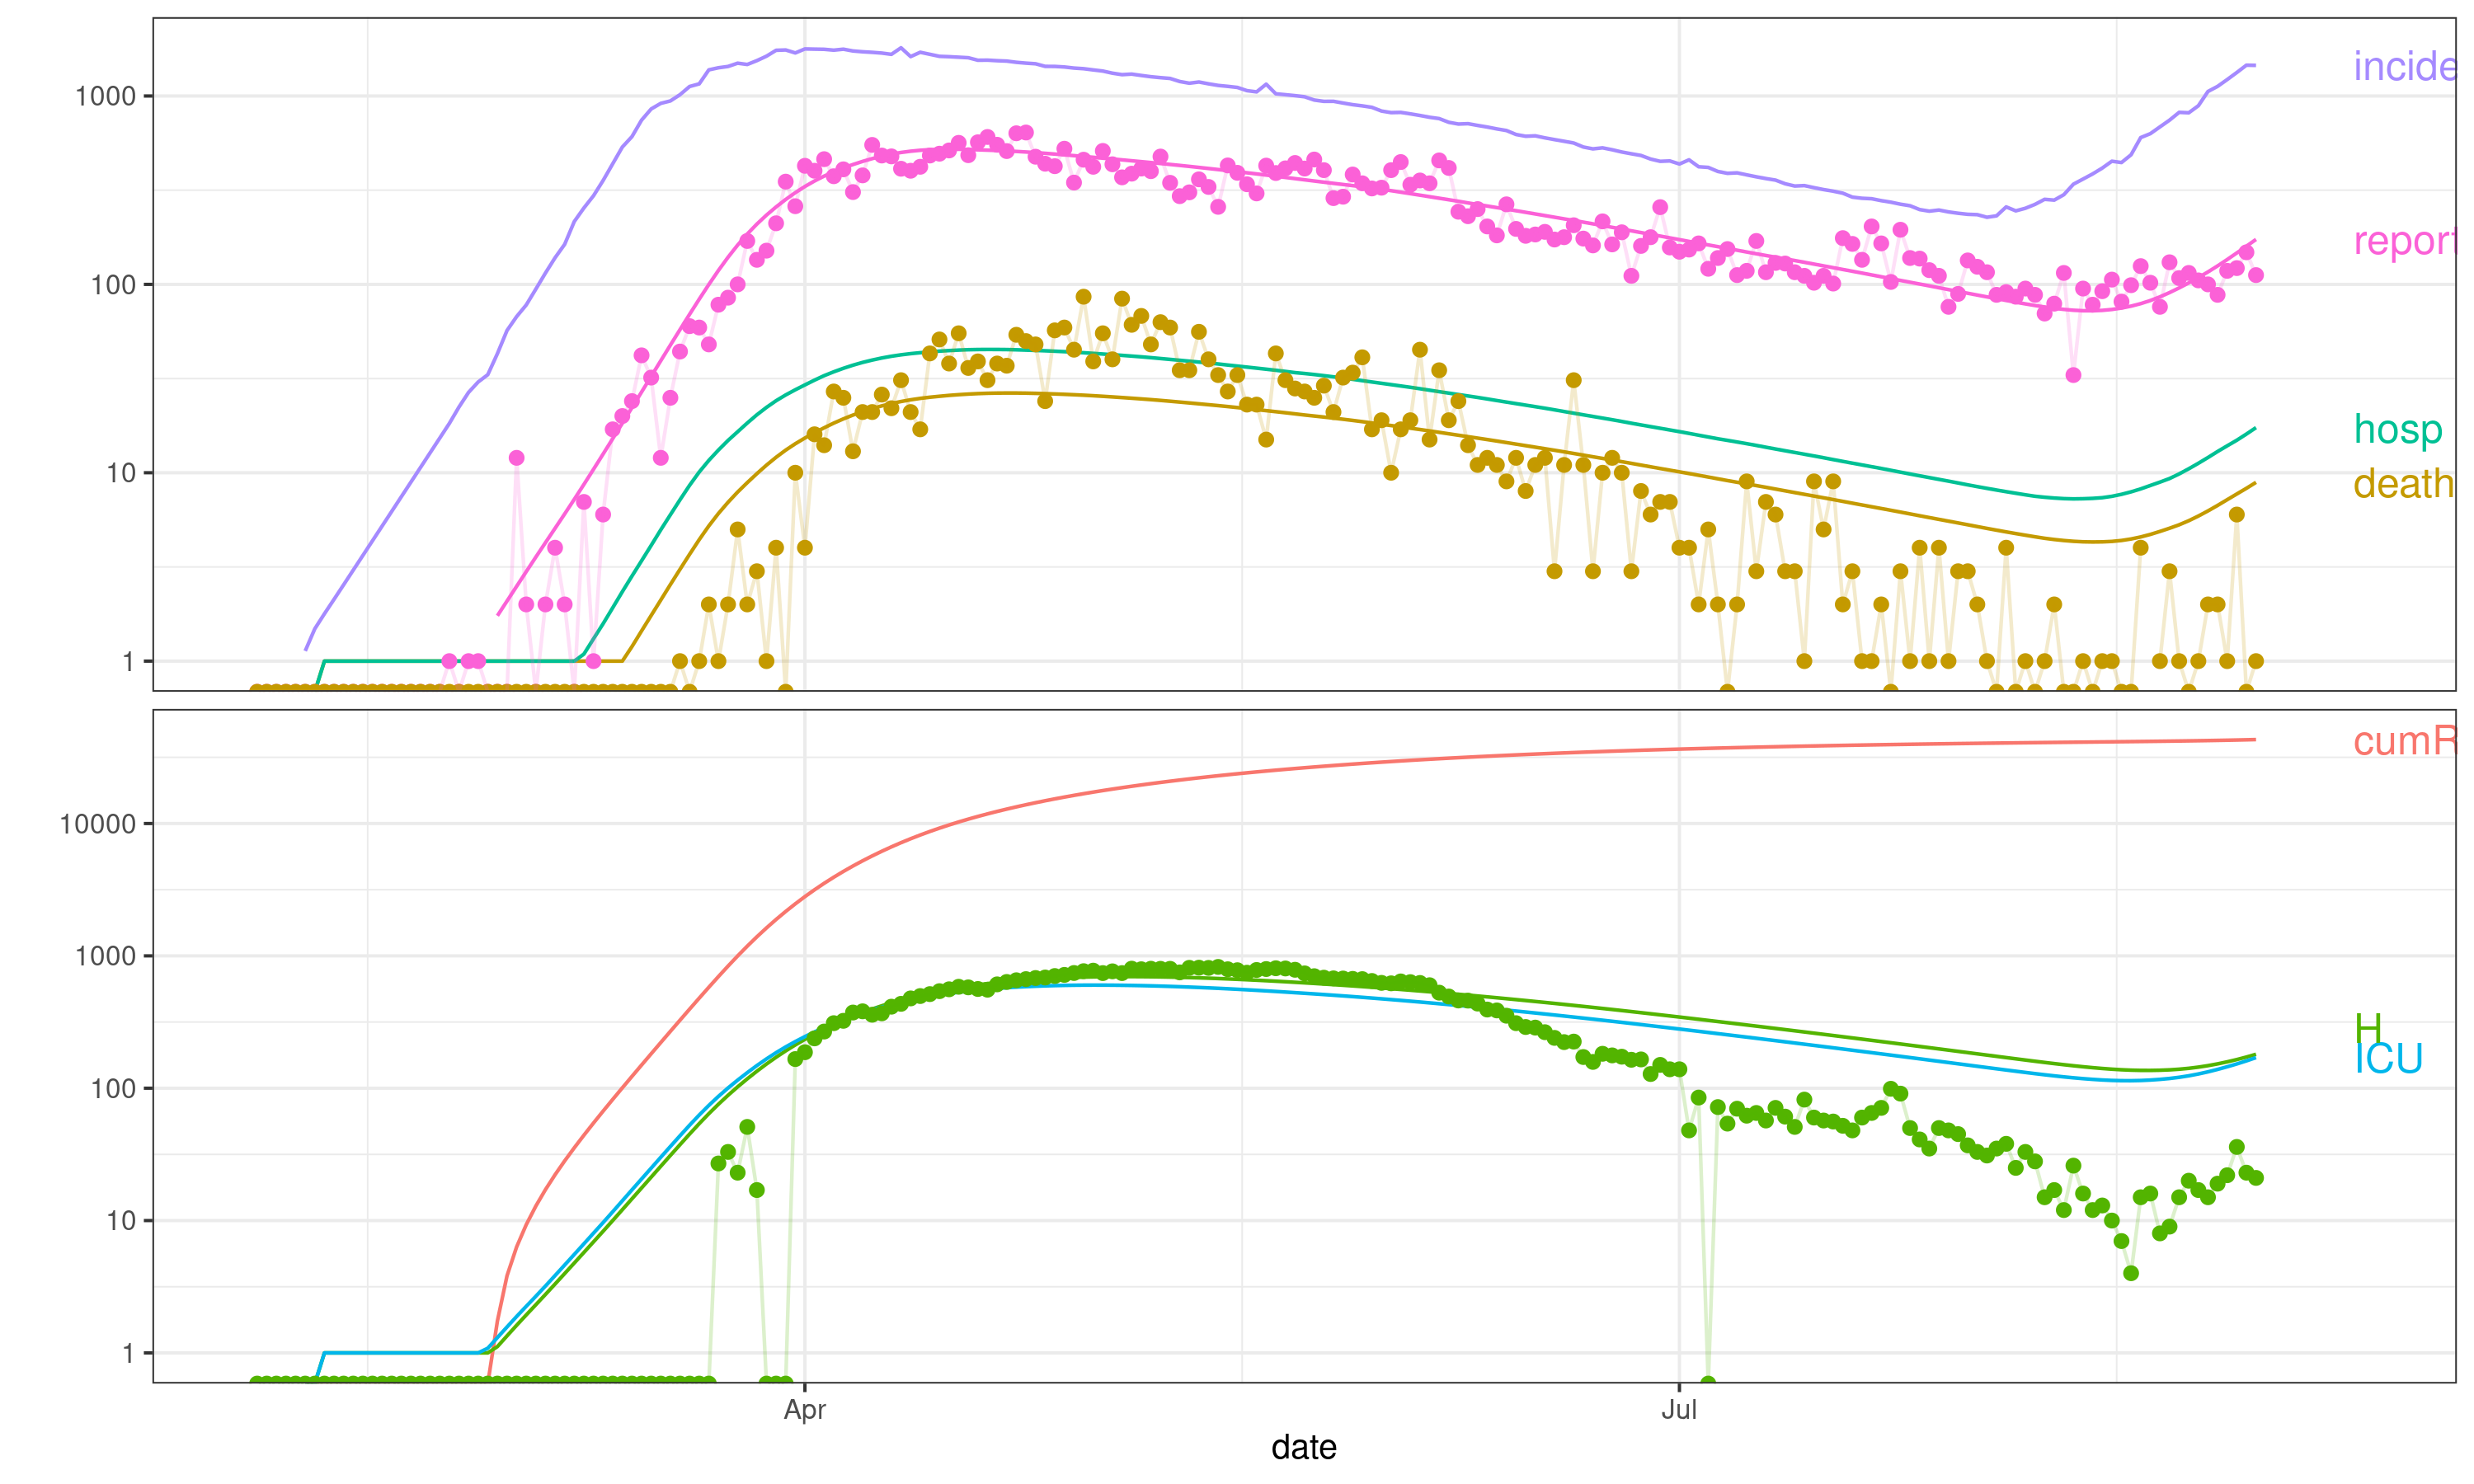
\includegraphics[width=\maxwidth]{figure/ontario_base.png}

\caption{Ontario calibration}
\label{fig:Ont_calibration}
\end{figure}

\begin{figure}[ht!]
\definecolor{shadecolor}{rgb}{0.969, 0.969, 0.969}\color{fgcolor}
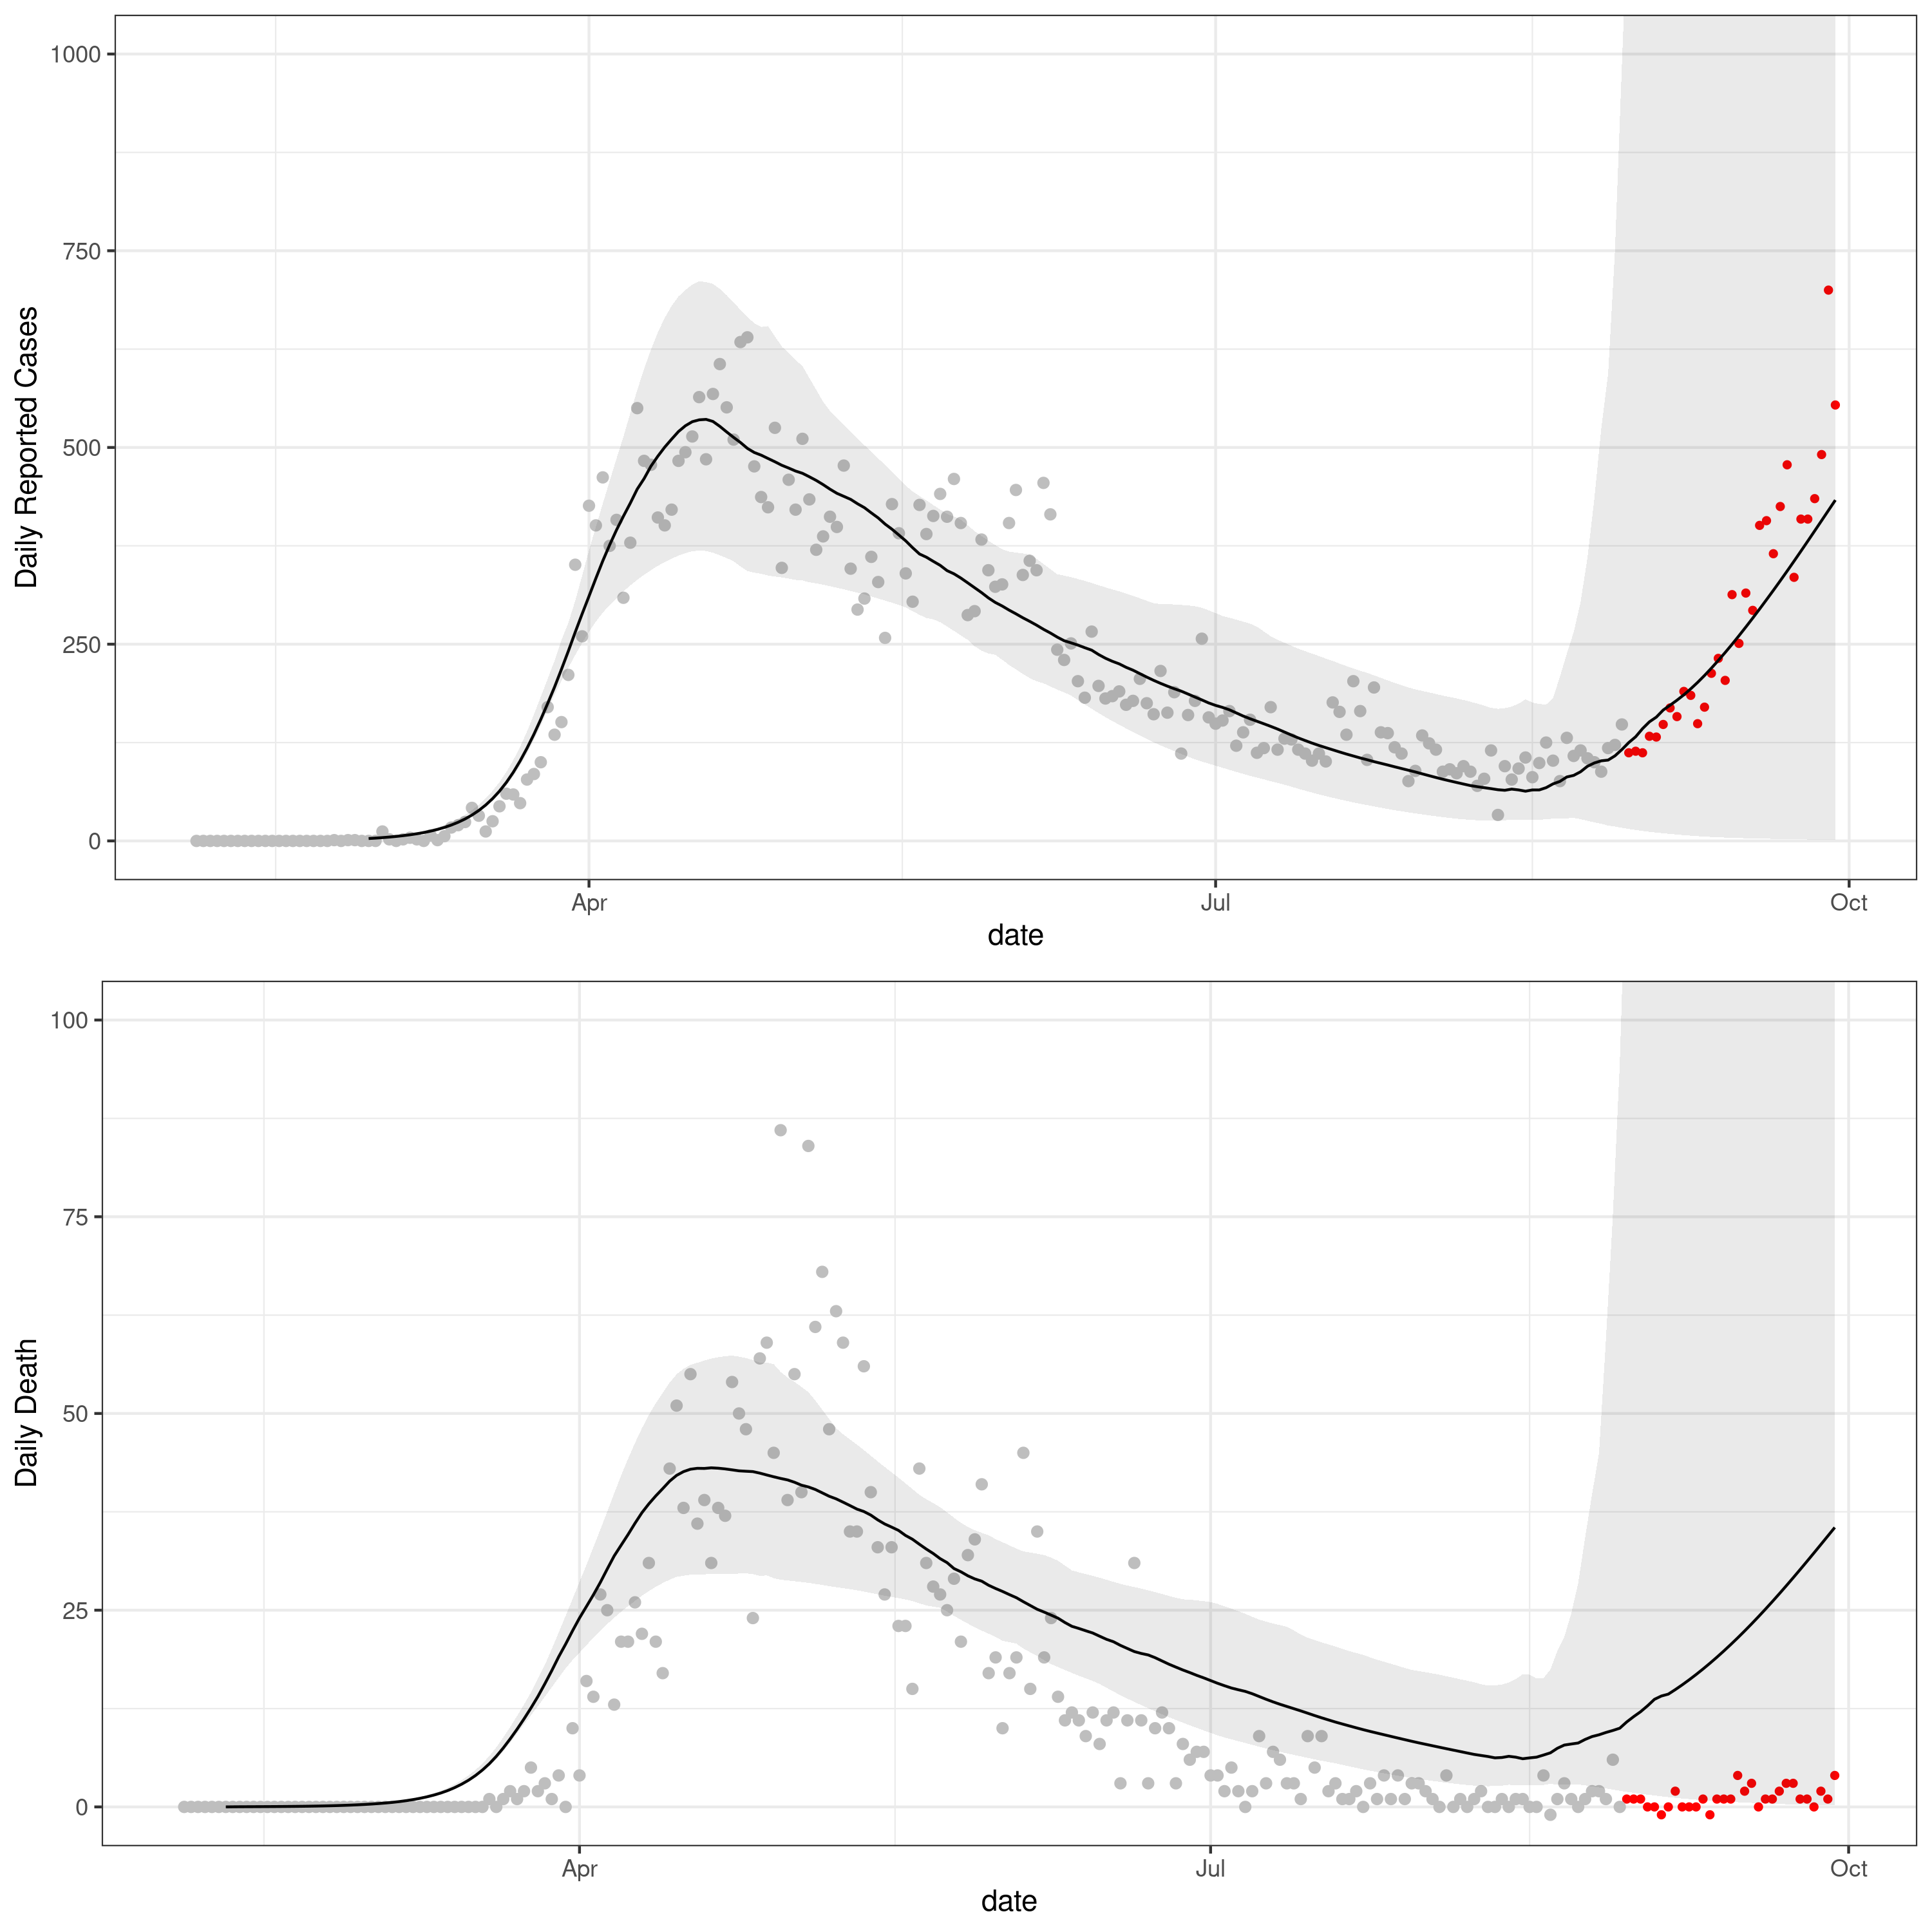
\includegraphics[width=\maxwidth]{figure/ontario_base_forecast.png}

\caption{Ontario base forecast}
\label{fig:Ont_calibration_base_forecast}
\end{figure}

\begin{table}
\centering
\input{"base_table.tex"}
\caption{Parameter estimates for base model calibration}
\label{table:base}
\end{table}


\FloatBarrier

\subsection{Testify}

The base model is relative simple but does not account for testing practices. Testing strategies are constantly changing over the course of the pandemic due to supply and demand of the labs and mandates for lifting restrictions. Figure \ref{fig:Ont_testing} shows the daily testing in Ontario in the calibration time frame. The verticle line is the cut-off between the calibration window (before September 1st 2020) and 30 days ahead for the forecast window. The testing intensity over the forecast window is assumed to be constant as the last observed testing intensity on August 30th 2020.  


\begin{figure}[ht!]
\definecolor{shadecolor}{rgb}{0.969, 0.969, 0.969}\color{fgcolor}
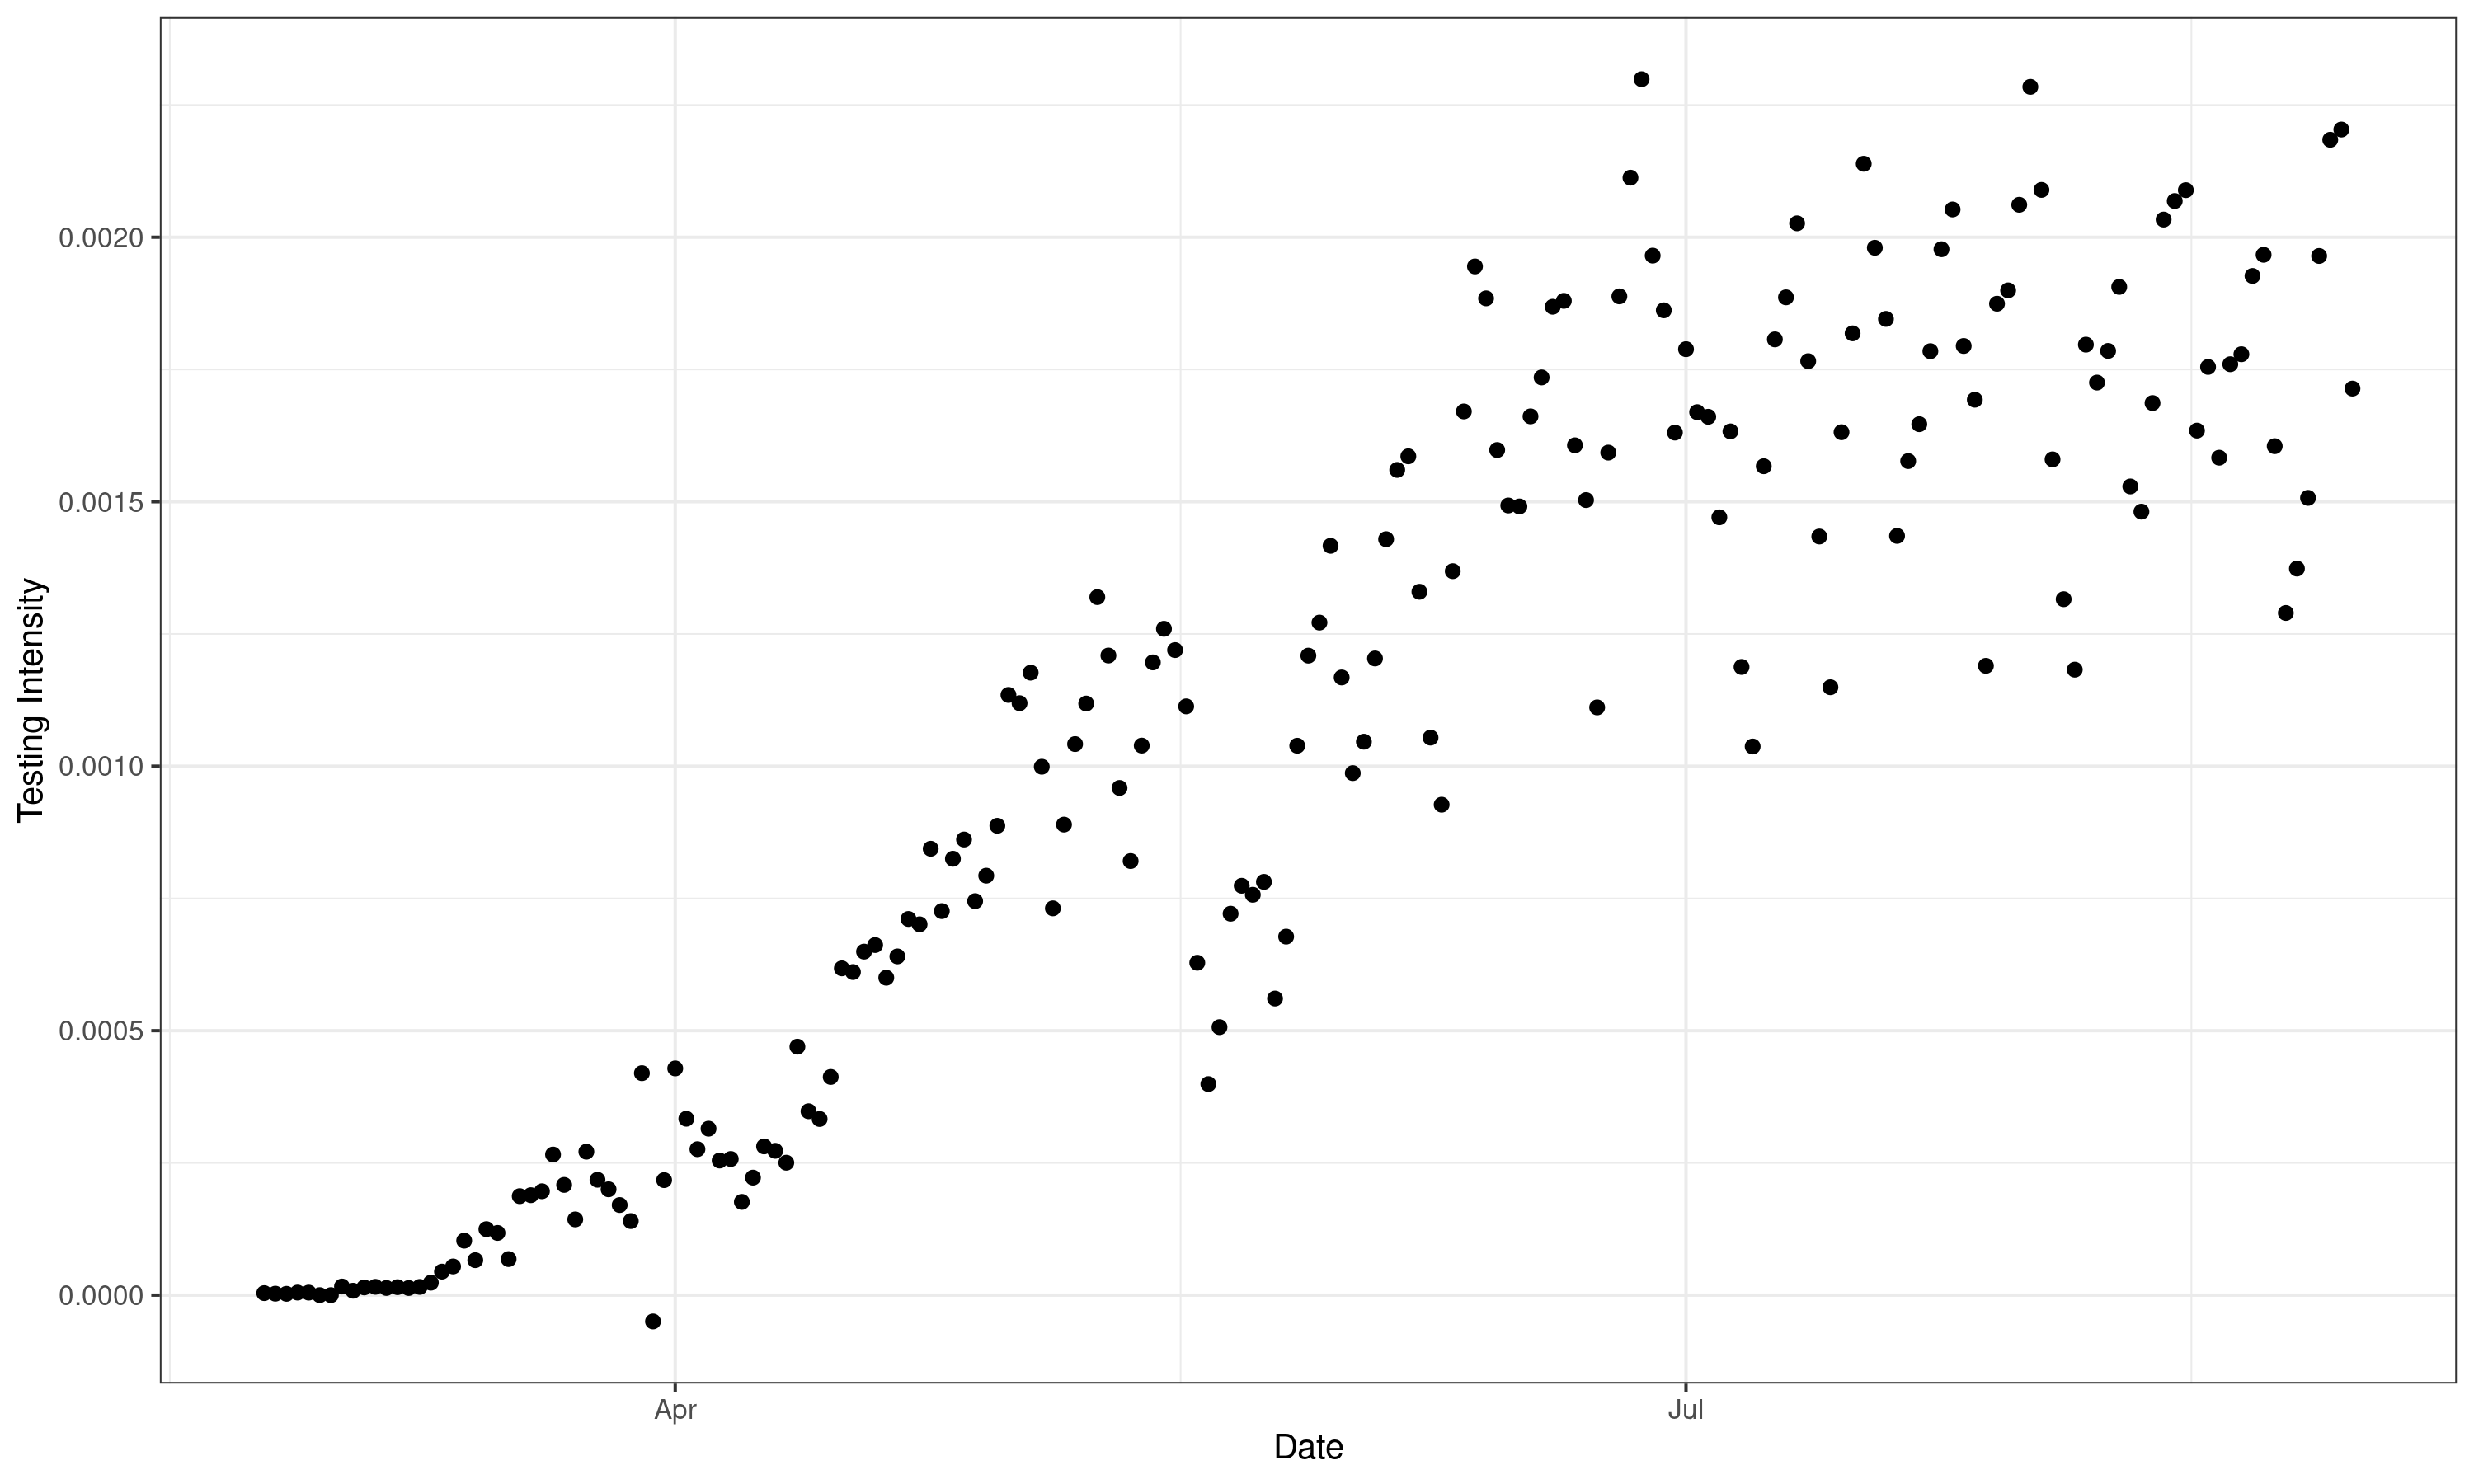
\includegraphics[width=\maxwidth]{figure/ontario_testing.png}


\caption{Ontario Testing Intensity}
\label{fig:Ont_testing}
\end{figure}

\FloatBarrier

Figure \ref{fig:Ont_calibration_testify} shows the calibration account for testing. 
Compared to the reports fit from the base model, the testify fit is much more noisy which corresponse to the noise in observed testing intensity. 
Unlike, the base model, when we control for testing, it will provide a more realistic estimate of the real effect of changes in transmission.
\mike{todo: does this make sense? compare mobility parameters?}.

\begin{figure}[ht!]
\definecolor{shadecolor}{rgb}{0.969, 0.969, 0.969}\color{fgcolor}
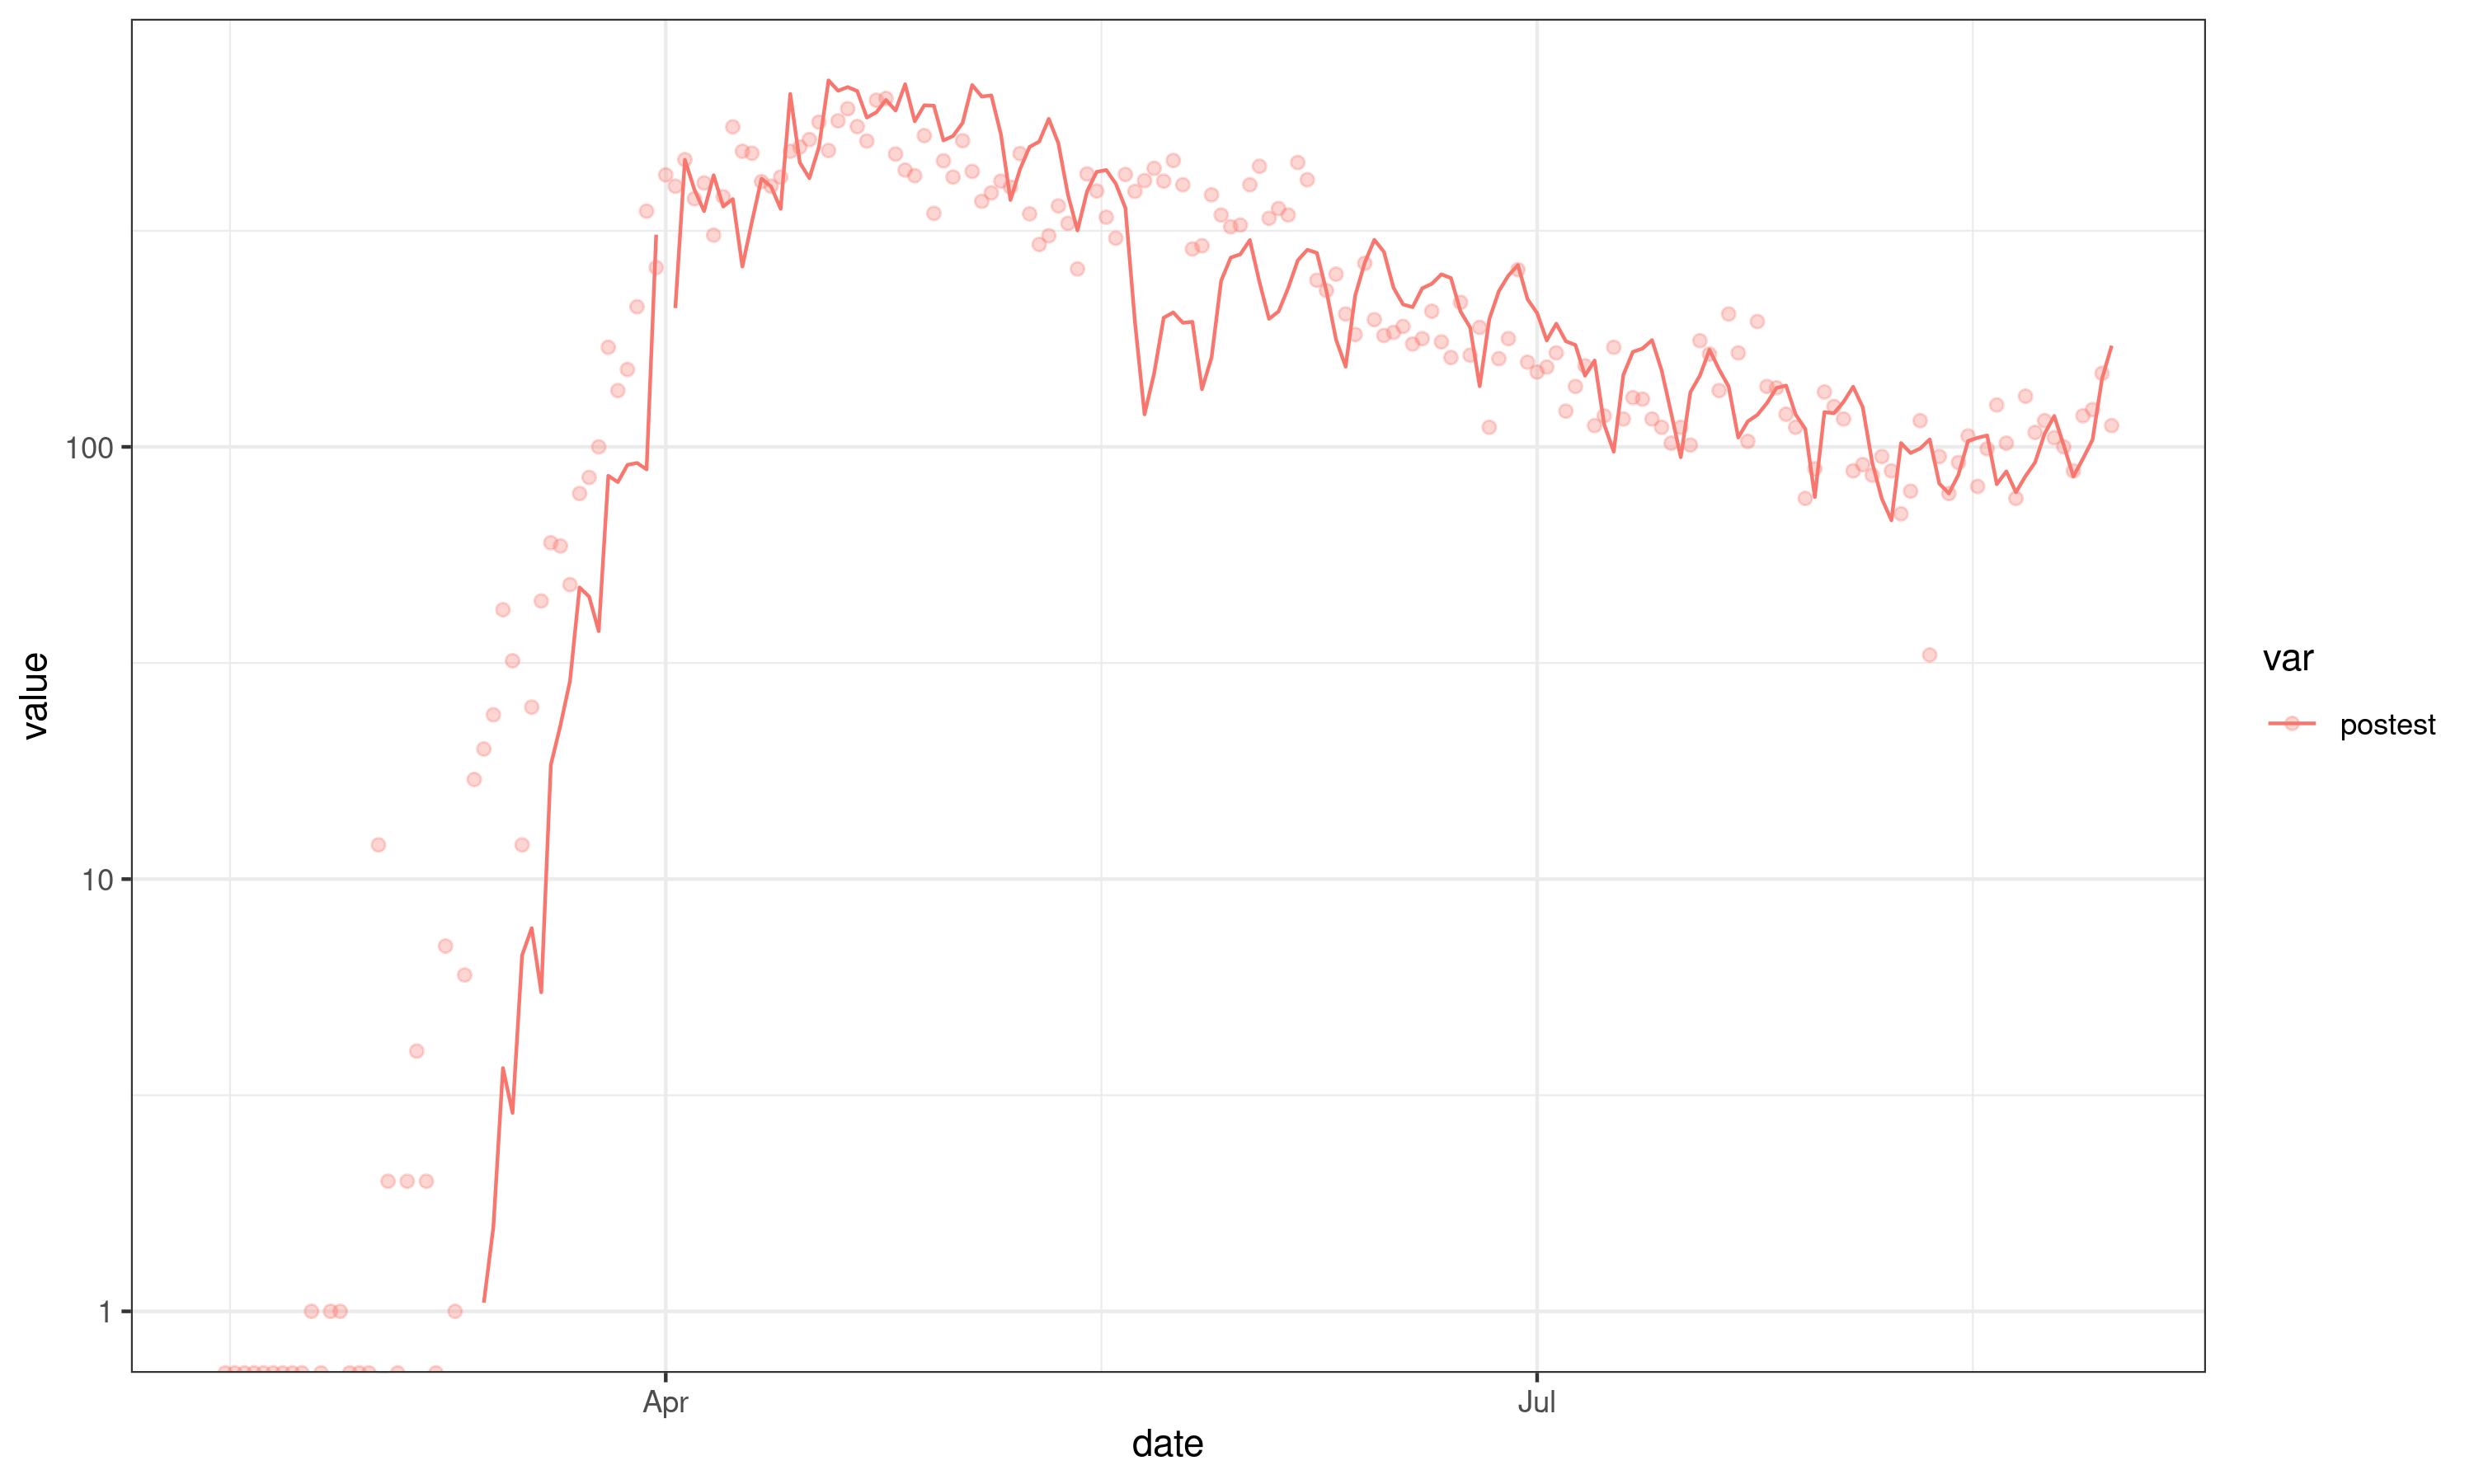
\includegraphics[width=\maxwidth]{figure/ontario_testify.png}

\caption{Ontario Testify}
\label{fig:Ont_calibration_testify}
\end{figure}

\begin{figure}[ht!]
\definecolor{shadecolor}{rgb}{0.969, 0.969, 0.969}\color{fgcolor}
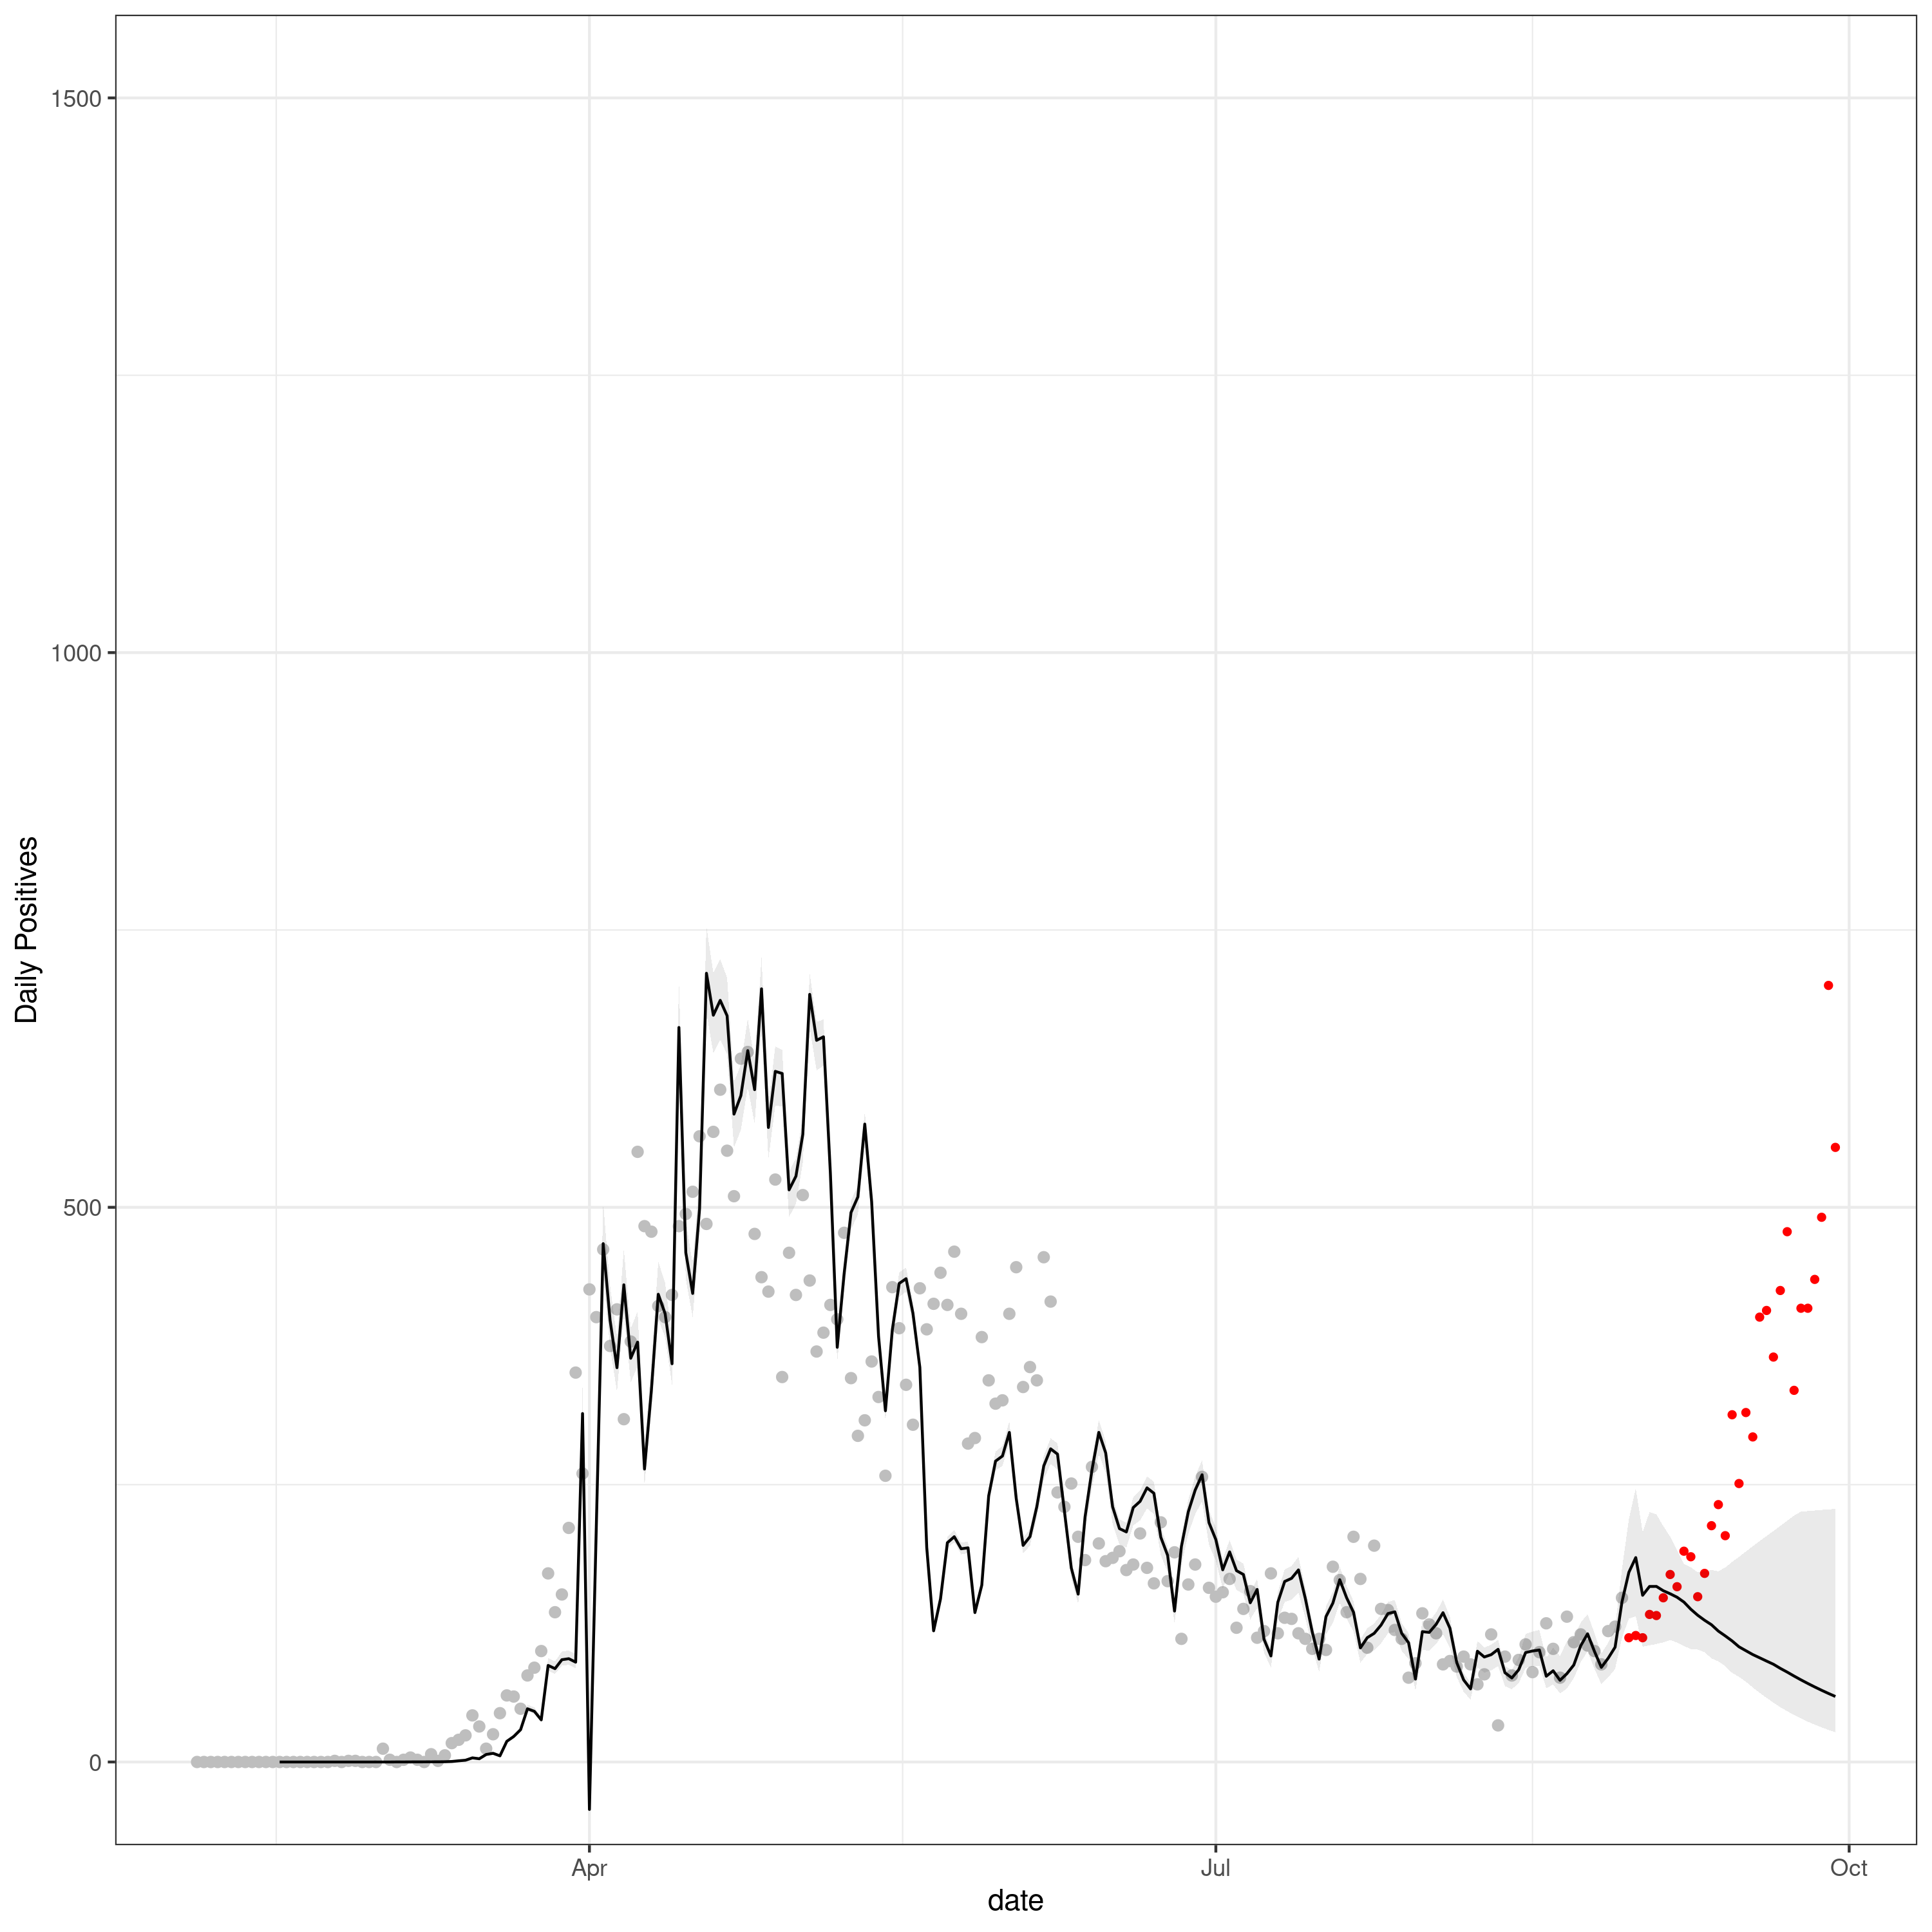
\includegraphics[width=\maxwidth]{figure/ontario_testify_forecast.png}

\caption{Ontario Testify}
\label{fig:Ont_calibration_testify_forecast}
\end{figure}

\mike{We (I) probably should make another forecast using the testing intensity of the forecast window. Thoughts?}

\begin{table}
\centering
\input{"testify_table.tex"}
\caption{Parameter estimates for testify model calibration}
\label{table:testify}

\end{table}

\FloatBarrier

\section{Discussion}

We have fitted two models varying in complexity to SARS-CoV-2 daily reporting and death time series data for Ontario Canada from March 1st to Aug 30th 2020. 
The simple base model is the typical simplistic type of compartmental epidemic model to infectious disease epidemics. 
The testify model is a practical addition to the base model that allows the model to cooperate with different testing practices and policy changes.

\subsection{Limitations}

Our model assumes homogeneous mixing of the population. 
No age-related or spatial contact structure is considered. 
We did not include hospitalization in the calibrations due to reporting from capacity issues which became a serious issue with the admissions and occpuancy underreporting the severity of the pandemic.
In addition, long-term care facilities (LTCFs), where many elderly people in Canada have died without going to hospital, have not been modelled explicitly.  
While we do not anticipate any qualitative differences in results, explicitly creating compartments and calibrating to data for LTCFs would likely allow us to match ICU occupancy and forecast
pressure on ICUs more accurately but will not resolve the issues on hospital intensity. 

\subsection{Conclusions}

SARS-CoV-2 continues to be a global burden after 3 years. 
Here we demonstrated a simple modeling framework that can flexibly fit epidemic data and easily allow additional complexities to account for features during the epidemic. 
We learned two things about fitting epidemic data. 
First, it is important to have ways to incorporate time-varying parameterizations fitting changes in the observed data or behavioural changes. Time-varying transmission rates played an important role in our calibration. 
Second, allowing for testing intensity to disaggregate the transmission rates through time (i.e. does increase in positive cases/confirmation due to an increase in transmission or testing capacity). 
The flexibility of incorporating various time-vary parameterizations allows users to make more realistic features and scenario exploration. 

%%\input{nextsteps.tex}

\clearpage

% \section{Appendix: Model calibrations for each province}\label{sec:supp}
% 
% Our fits are shown in the \hyperlink{current.fits}{following pages},
% with one page per province.  Provinces are ordered by total
% population. The smaller provinces (later pages) have far fewer cases
% so the fits are less reliable.
% 
% The data to which we calibrated the model are shown with dots.
% We fitted to hospital occupancy rather than admissions because
% we have admissions data only for Ontario.  The fitted model
% is shown with solid curves in each panel.
% The bottom row shows inferred total disease incidence,
% and
% our mobility index for the province.
% \david{[temporarily deleted because we don't have $\R_t$ in the plots]
% , and our inferred value of \Rt. Note that in our current model \Rt depends
% \emph{only} on the mobility index, the time period (early or late) and
% the direct and indirect effects of susceptible depletion.}
% 
% \FloatBarrier
% \clearpage

%% LOOP THROUGH PROVINCES TO GET FIGURES:
%% Note that we could implement a switch for the captions via:
%%   https://tex.stackexchange.com/questions/64131/implementing-switch-cases

\clearpage

\bibliographystyle{vancouver}
\bibliography{McMasterReport}

\end{document}
